\chapter{Hintergrund}
\label{chap:background}

Um in der weiteren Arbeit den Konsistenzvergleich zwischen BPMN- und BROS-Modellen durführen zu können, werden zunächst die Modelle und ihre unterstützten Elemente vorgestellt.
Dafür wird wird für jedes Modell ein Metamodell eingeführt.
Da sich einige Namen zwischen den Modellen doppeln werden die Elemente der Metamodelle mit dem Präfix "Bpmn" bzw. "Bros" benannt.

\section{Business Process Model and Notation}

Die \emph{Business Process Model and Notation} (\textbf{BPMN}) ist der Standard für die grafische Beschreibung von Geschäftsprozessen.
Dabei wird das Verhalten eines Systems mit einer an Flussdiagrammen angelehnten Form beschrieben.
Einer der Hauptvorteile von BPMN ist die große Verbreitung.
Dank ihr können Prozessbeschreibungen auf einfache Art und Weise zwischen verschieden Plattformen und Stackholdern ausgetauscht werden.
Neben der informellen Beschreibung von Prozessen unterstützt BPMN auch die direkte Ausführung von Geschäftsprozessen.
Mittels diverser Interpreter können in BPMN modellierte Abläufe zur Automatisierung einfacher Aufgaben oder ganzer Fertigungsprozesse genutzt werden.
Die Hauptelemente von eines BPMN-Modelles sind:

\begin{itemize}
    \item \textbf{Activity:} 
    Eine Activity beschreibt eine Tätigkeit die innerhalb des Geschäftsprozesses ausgeführt wird.
    Da eine Aufgabe ausgeführt wird, kann die Ausführung einer Activity längere Zeit in anspruch nehmen.
    Zur Darstellung wird ein Rechteck mit abgerundeten Ecken verwendet.
    \item \textbf{Gateway:}
    Ein Gateway wird für die Steuerung des Kontrollflusses verwendet. 
    An einem Gateway können verschiedene Kontrollwege zusammenlaufen oder sich teilen. 
    Dabei werden verschiedene Arten, wie zB. AND- und OR-Gateways unterstützt. 
    Dargestellt wird ein Gateway mittels einem um 45 Grad gedrehtem Quadrat. 
    \item \textbf{Event:}
    Ein Event beschreibt Ereignis das innerhalb des Geschäftsprozesses auftreten kann und werden mit einem Kreis dargestellt.
    Sie beeinflussen den Kontrollfluss, können ihn starten, pausieren oder auch beenden.
    Events werden in drei verschiedenen Dimensionen eingeteilt, nach ihrer Position, nach ihrer Wirkung und nach ihrer Art.
    Für die weitere Arbeit ist nur die Unterteilung nach ihrer Position innerhalb des Geschäftsprozesses wichtig.
    Dabei wird zwischen einem StartEvent (einfacher Rahmen), einem IntermediateEvent (doppelter Rahmen) und einem EndEvent (dicker Rahmen) unterschieden.
    \item \textbf{Flow:}
    Ein Flow ist eine gerichtete Verbindung zwischen anderen Modellelementen.
    Dabei wird zwischen SequenceFlows und MessageFlows unterschieden.
    Ein SequenceFlow stellt den Kontrollfluss dar und verbindet Elemente um eine Ausführungsreihenfolge festzulegen.
    Ein MessageFlow verbindet unterschiedliche Teilnehmer des Geschäftsprozesses und stellt die austausch von Mitteilungen dar.
    \item \textbf{Pool:}
    Ein Pool stellt eine Gruppe von zusammengehörenden Teilnehmern innerhalb eines Geschäftsprozesses dar.
    Dargestellt wird ein Pool mit einem Rechteck wobei der Name am linken Rand steht.
    \item \textbf{Swimlane:}
    Eine Swimlane ist ein einzelner Teilnehmer der zu einem Pool gehört und Aufgaben aus dem Geschäftsprozess erfüllt.
    Bei einem Pool der nur aus einer Swimlane besteht kann die Swimlane mit dem Pool vereinigt werden.
    Innerhalb eines Pools wird die Simelane als eine horizontale Bahn dargestellt.
    \item \textbf{Process:}
    Der Process bildet den vollständigen Geschäftsprozess ab und ist das Containerelement für die anderen Modellelemente.
\end{itemize}

Da BPMN schon längere Zeit in Benutzung ist hat es eine gute Toolunterstützung für die Modellierung.
Eines dieser Tools ist bpmn.io\footnote{https://demo.bpmn.io/}.
Es ist ein webbasiertes Tool das einen großteil des BPMN-Standards unterstützt.
Das Tool speichert und lädt die BPMN-Modelle in einem auf XML-basierenden Format mit der Dateiendung \emph{.bpmn}.
Die Datenstruktur basiert auf dem Metamodell das von der \emph{Object Management Group}\footnote{https://www.omg.org/spec/BPMN/2.0/About-BPMN/} spezifiziert wurde.

\begin{figure}
    \centering
    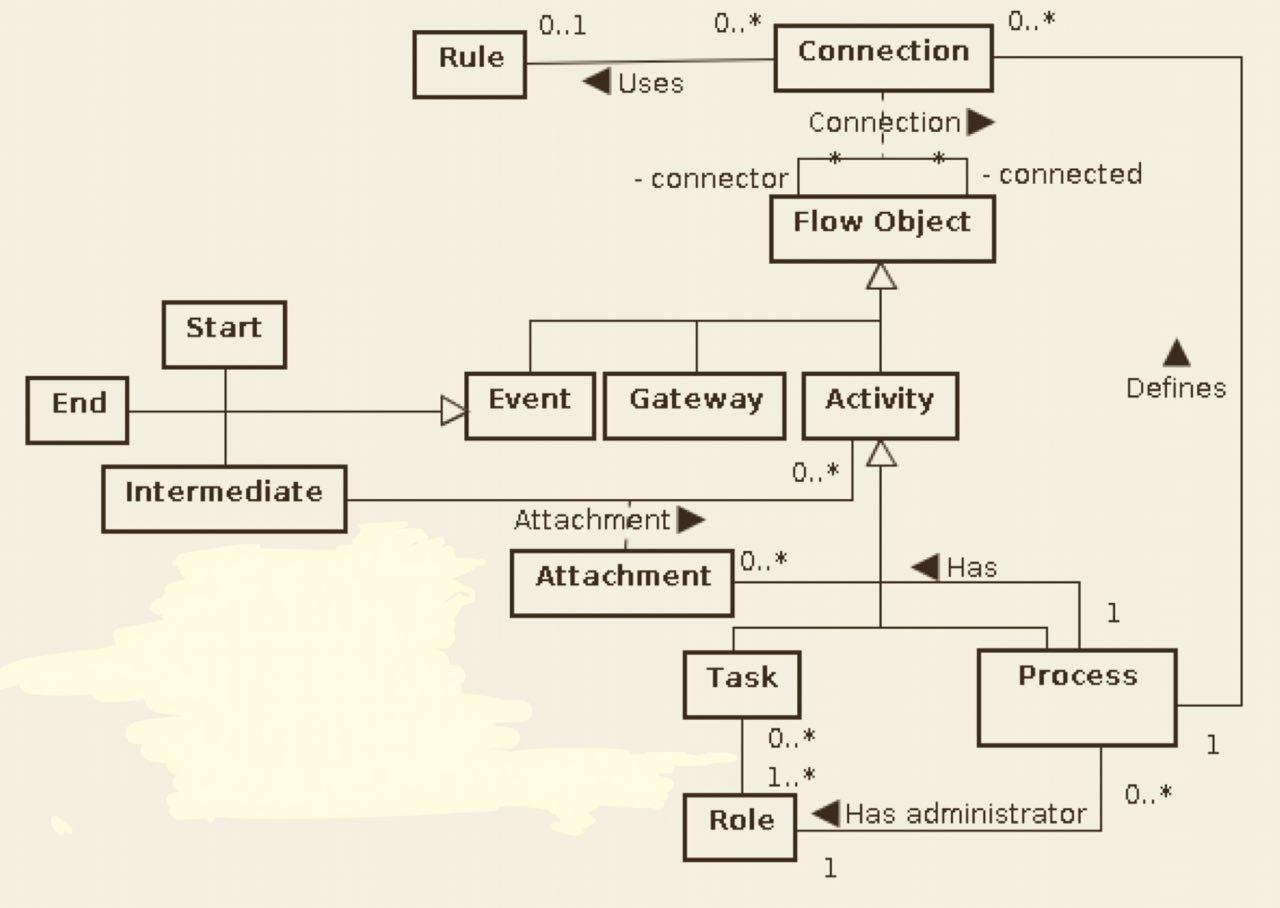
\includegraphics[width=\textwidth,keepaspectratio]{../images/bpmnMetamodell.jpg}%
    \caption{BPMN Metamodell}%
    \label{fig:bpmnMetamodell}
\end{figure}

Für die weitere Arbeit wird nur ein Teil des vollständige BPMN-Standards der \emph{OMG} genutzt.
Ein deutlich gekürztes Metamodell für Business Prozesse wurde von \cite{Loja2010} erstellt.
Das hier verwendete Metamodell basiert auf den Metamodellen der \emph{OMG} und von \cite{Loja2010} (vgl. \cref{fig:bpmnMetamodell}).
Es unterstützt dabei nur die oben genannten BPMN-Elemente.
Weitere BPMN-Elemente werden in dieser Arbeit und dem später entwickeltem Tool nicht betrachtet.

Mit dem BPMN-Metamodell aus \cref{fig:bpmnMetamodell} wird ein BPMN-Modell in einem Graphen, genauer einem Baum mit Querverweisen, dargestellt.
Die Wurzel des Baumes ist das Modell ansich.
Dieses kann mehrere Prozesse (BpmnProcess) enthalten.
Jeder Prozess beinhalten verschiedene Flowobjekte, dazu zählen Events (BpmnEvent), Gateways (BpmnGateway) und Activities (BpmnTask).
Die Events teilen sich in drei Unterklassen auf, die Start-, Intermediate- und EndEvents (BpmnStartEvent, BpmnIntermediateEvent, BpmnEndEvent).
Außerdem kann ein Prozess mehrere Pools (BpmnLaneSet) und Swimlanes (BpmnLane) enthalten.
Hierbei ist zu beachten, das obwohl eine Swimlane auch Flowobjekte enthalten kann, das jedes Flowobjekt nur einen Container haben darf.
So kann ein Flowobjekt nicht gleichzeitig Kind eines Prozesses und einer Swimlane seien.
Jedes Kind einer Swimlane ist transitiv auch Kind von dem Elternprozess der Swimlane.
Die beiden Flow-Arten bilden die Querverweise innerhalb des Baumes.
Ein MessageFlow (BpmnMessageFlow) kann zwischen allen BPMN-Elementen gezeichnet werden, wird aber hauptsächlich nur für die Kommunikation zwischen Prozessen verwendet.
Der SequenceFlow (BpmnSequenceFlow) stellt den Ablauf innerhalb eines Prozesses dar und darf nur zwischen Flowobjekten existieren.

\section{Compartment Role Object Model}

Das \emph{Compartment Role Object Model} (\textbf{CROM}) ist eine Modellierungssprache für Rollenbasierte Systeme.
Eine Rolle beschreibt einen Aufgabenbereich der von verschiedenen Entitäten übernommen werden kann, man sagt die Entität spielt die Rolle.
CROM führt zusätzlich noch das \emph{Compartment} ein, das den Kontext der Rolle abbildet, in dem diese gespielt werden kann.
Dazu wird das Modell in drei logische Aspekte unterteilt, den Verhaltensaspekt, den Relationenaspekt und den Kontextaspekt.
Der Verhaltensaspekt beschreibt die Aktoren bzw Entitäten und die Rollen die von diesen gespielt werden können.
Der Relationenaspekt fügt zu den Rollen weitere Constraints und Verbindungsbeschreibungen hinzu.
Im dritten Aspekt, dem Kontextaspekt wird mittels der Compartments die Kontextabhängigkeit modelliert.
Die dafür genutzten Elemente sind:

\begin{itemize}
    \item \textbf{RoleType:}
    Eine RoleType ist die Darstellung einer Rolle.
    Sie wird mit einem abgerundeten Rechteck vergleichbar mit einer UML-Klasse dargestellt.
    Eine Rolle kann einer Entität zusätzliche Attribute und Methoden hinzufügen.
    \item \textbf{CompartmentType:}
    In einem CompartmentType bildet den Kontext von verschiedene RoleTypes ab.
    Das Compartment ist an sich auch eine Rolle und kann von Entitäten gespielt werden.
    Graphisch wird es wie eine UML-Klasse dargestellt, die zusätzlich noch ein weiteres Feld für die beinhalteten Rollen besitzt.
    \item \textbf{NaturalType:}
    Ein NaturalType oder auch DataType stellt eine Entität bzw Aktor des Modelles dar.
    Sie unterschieden sich nur in der Semantik.
    Der NaturalType bildet eine natürliche Person ab, wohingegen der DataType einen künstlichen Teilnehmer beschreibt.
    Dabei werden beide Arten mit einer UML-Klasse dargestellt. 
    \item \textbf{Fulfillment:}
    Ein Fulfillment ist eine Relation die eine Entität mit einer Rolle oder einem Compartment verbindet.
    Sie beschreibt welche Rolle von welchen Entitäten gespielt werden kann.
    Damit ist das Fulfillment immer von einer Entität auf eine Rolle gerichtet.
    \item \textbf{Relationship:}
    Eine Relationship ist eine Relation zwischen Entitäten oder Rollen die mit einer einfachen Linie ohne Pfeilenden dargestellt wird.
    Sie kann je nach Annotierung ein Constraint oder auch eine Verbindung zwischen diesen beschrieben.
    \item \textbf{Package:}
    Ein Package hilft bei der Strukturierung von großen Modellen.
    In ihnen kann ein Submodell abgebildet werden, in das nur Relationen hinein, aber nicht hinaus führen dürfen.
\end{itemize}

CROM besitzt mit dem Eclipse Plugin \emph{FRaMED-2.0}\footnote{https://github.com/Eden-06/FRaMED-2.0} einen eigenen graphischen Editorsupport.
Der Name des Editors ist ein Akronym für \emph{Full-fledged Role Modeling EDitor} und wurde speziell für CROM entwickelt.

\section{Business Role-Object Specification}

Der neu entwickelte Ansatz der \emph{Business Role-Object Specification} (\textbf{BROS}) kombiniert die Vorteile der strukturbasierten Modellierung und der verhaltensbasierten Modellierung.
Als Grundlage für BROS dient die strukturbasierte Modellierungssprache CROM.
Diese wird mit Hilfe von Events um den Verhaltensaspekt erweitert.
Zusätzlich zu den CROM-Elemente werden folgende Modellelemente unterstützt.

\begin{itemize}
    \item \textbf{Scene:}
    Eine Scene stellt einen Teilnehmer innerhalb eines Prozesses dar.
    Sie besitzt Methoden und kann Rollen, Events und andere Scenen beinhalten.
    Dargestellt wird sie mit einem Rechteck mit doppeltem linkem Rahmen.
    \item \textbf{Event:}
    Ein Event beschreibt ein Ereignis innerhalb des Geschäftsprozesses.
    Mit einem Event kann eine Rolle erzeugt bzw. beendet werden.
    Dabei kann ein Event eine beliebige Abstraktion eines Prozesses sein.
    \item \textbf{Create-/DestroyRelation:}
    Eine Create- bzw. DestroyRelation verbindet ein Event mit einer Scene oder Rolle.
    Sie beschreibt welches Event für das erstellen oder das auflösen einer Rolle im Geschäftsprozess verantwortlich ist.
    Eine CreateRelation ist von einem Event zu einer Rolle/Scene gerichtet, eine DestroyRelation verläuft in die gegensätzliche Richtung.
    \item \textbf{ReturnEvent:}
    Ein ReturnEvent ist ein Event, welches die aktuelle Scene beendet.
    Es wird als ein Event mit doppeltem Rahmen auf dem Rand der Scene dargestellt.
    Das ReturnEvent ist nicht mit einer DestroyRelation verbunden, da es implizit im gesamten Verlauf der Scene auftreten kann.
\end{itemize}

Auch BROS besitzt mit \emph{FRaMED.io}\footnote{https://eden-06.github.io/FRaMED-io/} Editorsupport.
\emph{FRaMED.io} ist eine Neuentwicklung von \emph{FRaMED-2.0} und wie \emph{bpmn.io} webbasiert.
Damit ist es Plattformübergreifend, ohne aufwendige Installation nutzbar.

\textit{TODO}

\begin{figure}
    \centering
    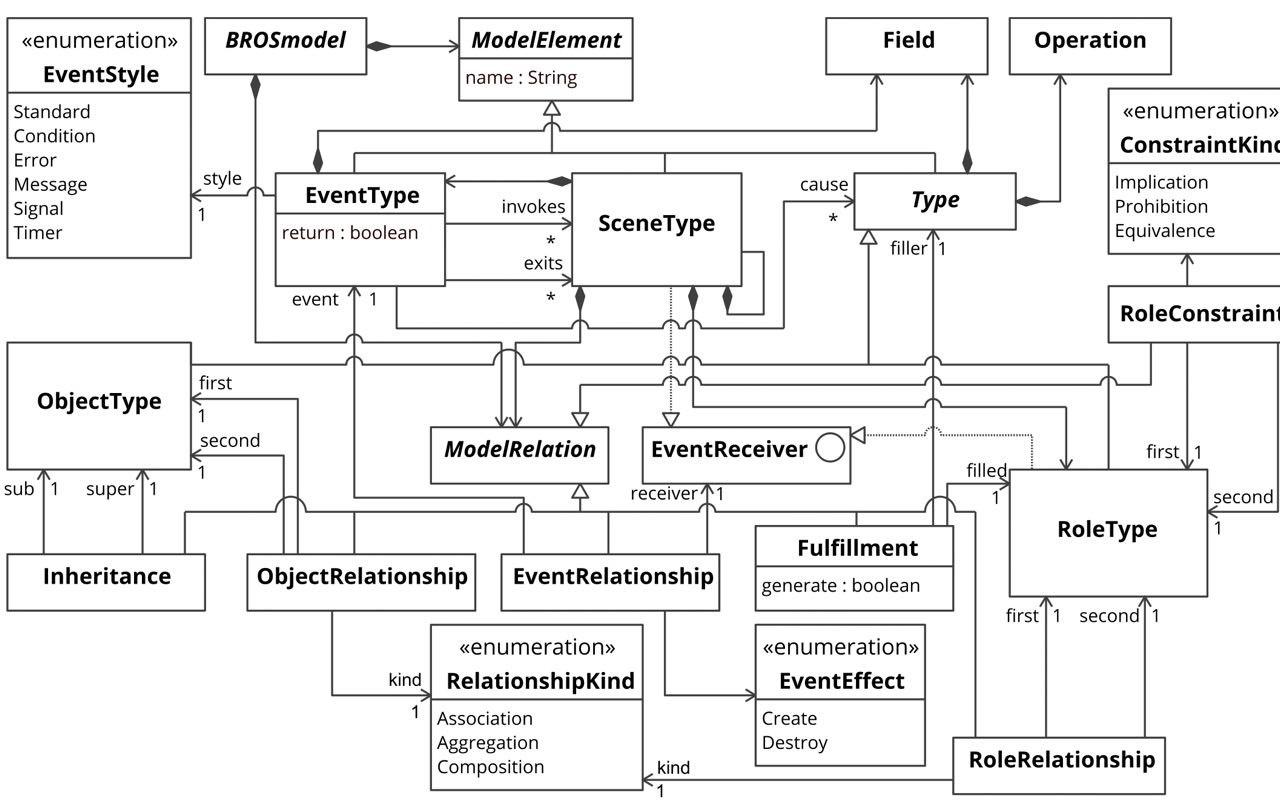
\includegraphics[width=\textwidth,keepaspectratio]{../images/brosMetamodell.jpg}%
    \caption{BROS Metamodell}%
    \label{fig:brosMetamodell}
\end{figure}

Das Metamodell in \cref{fig:brosMetamodell} basiert auf dem von \cite{Schoen} und dem in FRaMED.io implementierten Metamodell.
Die Eelemte des Metamodelles teilen sich in zwei Klassen auf.
Auf der einen Seite sind die Connections, zu denen die Create- und DestroyRelation (BrosCreateRelation, BrosDestroyRelation) gehören.
Auf der anderen Seite sind die Objekte die sich in Endknoten und Objektgruppen teilen.
Endknoten sind die NaturalTypes (BrosClass), die RoleTypes (BrosRoleType), Events (BrosEvent) und ReturnEvents (BrosReturnEvent).
Die Objektgruppen sind Containerelemente die andere Objekte enthalten können.
Zu ihnen zählen der CompartmentType (BrosCompartment), das Package (BrosPackage) und die Scene (BrosScene).
Auch dieses Metamodell entspricht einem Graphen, genauer einem Baum mit Querverweisen.
Jedes Objekt darf nur Kind einer Objektgruppen seien und die Eltern-Kind-Beziehung ist transitiv.
Die Connections bilden die Querverweise innerhalb des Baumes.
